

\section{Project organization}
We decided to use the Scrum model for organizing our group. This ment that we had a flat organizational structure where everyone contributed with what they could. Even in a flat structure, it was important to share responsibilities, so each person of the group had a main focus area. If it was too much work for one person, it was important that the work was delegated to the others.

\subsection{Organizational diagram}
See figure \ref{fig:organizationalchart} below for an organizational diagram that shows the structure of our group internally, as well as our connection to our advisor and Thales. Notice that even though we had a project leader, he was at the same level as all the others. This was to indicate that the project leader was not the big boss . We were all equally responsible for this project being a success.
\begin{figure}[hbt]
\begin{center}
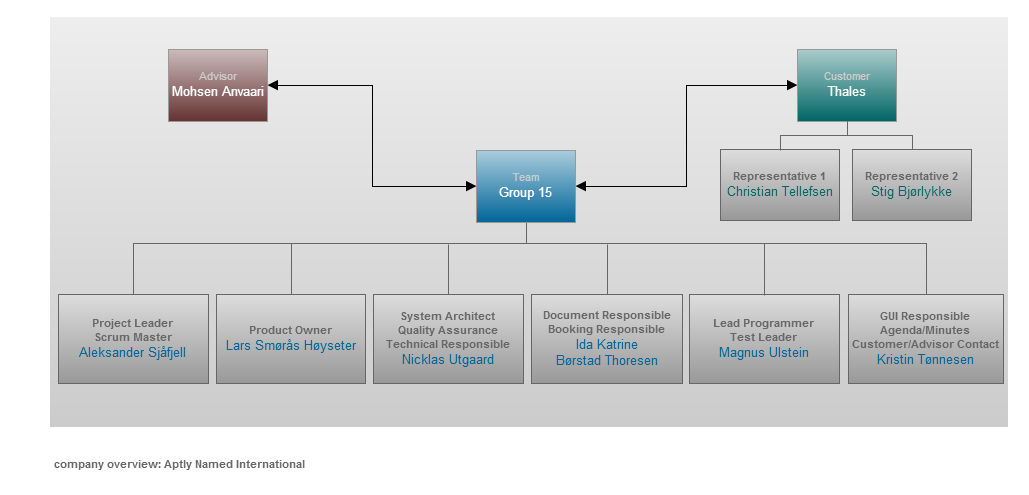
\includegraphics[width=\textwidth]{Organizational_Chart_v2}
\caption{Organizational chart} \label{fig:organizationalchart}
\end{center}
\end{figure}

\newpage

\subsection{Role allocation}
See table \ref{tab:roleallocation} below for a role allocation table that shows what roles each person had, as well as a short description of the role. The roles was merely a guideline on who were responsible for the depicted area. If the person needed more help, then we all contributed to get the result we wanted. We were all in this together.
\begin{table}[h!]
\begin{center}
\begin{tabularx}{\linewidth}{>{\setlength\hsize{.5\hsize}}X|>{\setlength\hsize{0.3\hsize}}X|>{\setlength\hsize{1\hsize}}X} \hline
\textbf{Role} & \textbf{Person} & \textbf{Responsibilities} \\ \hline \hline
Project leader & Aleksander & Make sure everybody does what they are supposed to and peacefully resolve disputes between participants \\  \hline
Scrum master & Aleksander & Make sure the team’s work conform to Scum standards and help the team do the best work possible \\ \hline
Booking of rooms & Ida & Booking rooms for the meetings and other activities \\ \hline
Agendas, minutes of meetings & Kristin \& Lars &Write agendas and minutes of meeting and send these out within the specified time limits \\ \hline
Customer/advisor contact & Kristin & Main contact person for customer and advisor \\ \hline
Document responsible & Ida &Keep track of what is to be contained in the project report, what has been written and what remains \\ \hline
Project report layout responsible & Ida &Find programs to make tables and graphs, and check that all diagrams are similar in style \\ \hline
System architect & Nicklas & Defining the system architecture \\ \hline
Test leader & Magnus & Lead the testing team \\ \hline
Technical responsible & Nicklas & Setup of Netbeans, Git and other tools that the team uses in the development \\ \hline
Quality assurance responsible & Nicklas & Make sure that all routines, templates and standards are followed \\ \hline
Responsible for graphical user interface & Kristin & Design the views and the interactions and setting up the MVC structure \\ \hline
Lead programmer & Magnus & Responsible for having a general overview of the code. This means knowing what is to be implemented next, and seeing that this is done at the right time \\ \hline
Product owner & Lars & Represent the stakeholders and ensure that the team delivers value to businesses\\ \hline
\end{tabularx}
\end{center}
\caption {Role allocation} \label{tab:roleallocation}
\end{table}

\newpage

\subsection{Weekly schedule}
See table \ref{tab:weeklyschedule} below for a weekly schedule that shows how we allocated time for the Customer Driven Project. As we all said how much we were able to contribute to the project, we must ensure that work outside of group work-hours was done to reach the goal.
\begin{table}[h!]
\begin{center}
\begin{tabular}{l|l|l|l|l|l} \hline
 & \textbf{Monday} & \textbf{Tuesday} & \textbf{Wednesday} & \textbf{Thursday} & \textbf{Friday} \\ \hline \hline
\textbf{08-09} &  & Group work &  &  &  \\
\textbf{09-10} &  & Group work &  &  &  \\
\textbf{10-11} &  & Group work &  &  &  \\
\textbf{11-12} &  & Advisor meeting & &  &  \\
\textbf{12-13} & Group work & Group work & Customer meeting &  &  \\
\textbf{13-14} & Group work & Group work & Group work &  &  \\
\textbf{14-15} & Group work & Group work & Group work &  &  \\
\textbf{15-16} & Group work &  & Group work &  &  \\
\textbf{16-17} & Group work &  & Group work &  &  \\
\textbf{17-18} & Group work &  & Group work &  & \\ \hline
\end{tabular}
\end{center}
\caption {Weekly schedule} \label{tab:weeklyschedule}
\end{table}


